\subsubsection{Motivations}
\label{sec:descriptor_motivation}

As can be seen from the discussions in the previous section, both the supervised and unsupervised ML are statistical methods that can be applied to facilitate us in exploring the chemical-structural-property relationships for materials, therefore, the prerequisite that will enable us in applying these statistical methodologies, as opposed to the traditional approach of establishing qualitative understanding via known descriptive physical laws, is to \textit{construct physically meaningful mathematical representations} to describe the chemical, physical and/or structural attributes of the material systems to be studied. Very often, these mathematical representations are cast into the form of high-dimensional vectors $\boldsymbol{\chi}\in\mathbb{R}^N$, which shall be referred interchangeably as either the \textit{feature vectors} or \textit{descriptors}, such that we can enrich the information content that has been encoded for a given material, so it can be maximally differentiated from other materials within the set of materials to be studied.


More specifically, for supervised ML [\cref{sec:supervised_ML}], the feature vector $\boldsymbol{\chi}$ served as the \textit{independent variable}, which, will fundamentally allow a (often highly non-linear) mathematical relationship to be established, that correlates the target property with the independent variable, enabling the fast predictions of materials properties with the trained model. On the other hand, in unsupervised ML [\cref{sec:unsupervised_ML}], we often consider $\boldsymbol{\chi}$ as the \textit{coordinates to locate materials in the high-dimensional space}, providing a `geographic' interpretation of the materials space, upon which we can discover trends, patterns and outliers, similar to how we can identify the spatial relationships amongst objects on the geographical maps based on the altitudes and latitudes.  

Depending on the nature of the specific task that one is aiming to solve, here, we consider two general strategies with which  the feature vectors can be constructed to enable efficient learning, namely a \textbf{property-oriented} and a \textbf{structure-oriented} approach. 

The property-oriented approach has been covered in considerable details in our discussions [\cref{sec:supervised_ML}] on the applications of supervised ML for material property predictions, for which the purpose of learning is to establish a cheap surrogate relationship that allow exotic target properties, which are expensive to compute, becomes predictable from a set of physical/chemical properties that are relatively inexpensive to compute or retrievable from some existing tabulated sources. To understand which set of properties will lead to accurate prediction, thus suitable to be used for constructing the feature vectors, often requires strong prior knowledge on the dominating physics that leads to the desired physical outcomes. This also implies that such a property-oriented approach for constructing the feature vectors is highly problem specific thus not necessarily leads to a generalise scheme for constructing this type of feature vectors. As such, we shall not focus on this aspect in this section.


The overarching goal of computational materials science, as demonstrated in this monograph, is to establish the critically needed chemistry-structure-property relationship to guide future materials design, starting from the information of the materials' chemistry and atomistic structures. One of the fundamental principle that underpins this concept is that \emph{ materials with similar structures $\mathbf{R}$ should possess similar properties $p$}, and our goal is here is try to achieve a mathematical way of expressing such a concept. In the framework of kernelised supervised ML [\cref{sec:supervised_ML}], the (dis)similarities in the materials properties, which are often scalar or vectorial quantities, can be easily computed using well-known distance metrics, such as the Euclidean distance $d_{ij}=\Vert p_{i}-p_{j}\Vert_2$ (typically for scalars) and the (normalised cosine distance $d_{ij}=\sqrt{1-\bm{p}_1\cdot \bm{p}_2/(\Vert \bm{p}_1\Vert_2\cdot\Vert \bm{p}_{2}\Vert_2)}$ (typically for vectors). However, how one could similarly quantify the (dis)similarity between two atomistic structures, are generally non-trivial. Traditionally, the Root-Mean-Square-Deviation (RMSD) between the atomic positions of two structures, after they become optimally aligned through rotations,\cite{coutsias2004using,chisholm2005compack} have been commonly used for structural comparisons, but such an approach often lacks generality. For examples, method developed for comparing molecular crystals\cite{chisholm2005compack} are typically confined to crystals with identical molecule(s) in the asymmetric unit, thus not helpful for identifying the trend for different molecules that may adopt similar crystal packing structures.\cite{yang2018large}

As such, the construction of structure-oriented approach for constructing the feature vectors, or most commonly known as the structural descriptors, to facilitate structure-based ML through, most importantly, the quantification of structural similarities, is highly desired for atomistic materials ML. Over the years, a wide range of structural descriptors have been proposed and tested, including internal coordinates\cite{pulay1979systematic,echenique2006definition},  bond-order parameters,\cite{steinhardt1983bond}  atom-centred symmetry functions,\cite{behler2011atom} permutation-invariant polynomials,\cite{braams2009permutationally} Coulomb (for molecules)\cite{rupp2012fast} and Ewald (for crystal) matrix,\cite{faber2015crystal} as well as the SOAP\cite{bartok2013representing} and atomic cluster expansion (ACE) descriptor.\cite{drautz2019atomic} Most importantly, the development of SOAP (and other related\cite{drautz2019atomic,behler2011atom,shapeev2016moment}) descriptors have emerged into a unified framework\cite{willatt2019atom} for constructing \textbf{physics-inspired symmetrised atom density field representations} for molecules and materials, which has been thoroughly reviewed in a recent monograph.\cite{musil2021physics} In addition to the demonstrated examples in the previous sections on the applications of SOAP descriptors in supervised and unsupervised ML, such a unified framework provide a useful guidance to extend the SOAP descriptor to account for, such as, chemical diversity,\cite{de2016comparing,willatt2018feature}  tensorial properties,\cite{grisafi2018symmetry} as well as long-range physics,\cite{grisafi2019incorporating} that are critical in materials modelling, and have been demonstrated\cite{nigam2022unified} on how the popular scheme of  message-passing NNs for quantum chemistry\cite{gilmer2017neural} can be united under the same abstract mathematical formulation using the Dirac (bra-ket) notation from quantum physics. 

 

Therefore, the focus of our discussion will be on the family of symmetrised atom density field representations. The rich set of existing literatures on this topic renders a mathematically detailed account here somewhat meaningless. Understanding how fundamental physical constraints, particularly symmetry, are incorporated into the SOAP descriptor, is important for the practitioners of ML/AI-driven computational materials science how these models lead to higher data efficiency, better ability for extrapolation, as well as model explainability. However, these knowledge are often embedded in lengthy mathematical derivations, which requires strong prior knowledge in topics such as tensor algebra, group and representation theories, which may not be trivial for most practitioners of materials modellings. 

Hence, following the style of the present monograph, we aim to strike here a balance between mathematical formality and intuitiveness to help readers to understand the most critical aspects behind the design of this group of structural descriptors, and building up linkages to AI models that are to be discussed in the subsequent sections.

\subsubsection{Coordinate Systems in Atomistic Modelling}\label{sec:coordinates_systems}


The starting point of any atomistic molecular/materials modelling is to provide the computer program with the structural (and chemical information) of the system being studied, and this structural information basically tells the computer program the position of each atom in the three-dimensional space $\mathbf{r}_i$ for each given atom $i$. Before we dive into the details of structural descriptor, we provide a brief account on the choices of coordinate systems that are common for atomistic modelling, and demonstrate why they are not suitable for the purposes of ML. Readers who are familiar with this topic may skip this section.

For molecular systems, the most intuitive choice to define $\mathbf{r}_i$ is to use the standard \textbf{Cartesian coordinates} system that define $\mathbf{r}_i\in\mathbb{R}^3$ as a three-dimensional vector quantity $\mathbf{r}_i=(x_i,y_i,z_i)$. The enumeration of $\mathbf{r}_i$ is thus clearly depends on the position of the origin and the orientations of the three orthogonal axes, referencing to which $\mathbf{r}_i$ is defined, thus it is non-unique, as  applying  a translational operation $\bm{t}$ to the coordinates ($\bm{r}^\prime\leftarrow \bm{r}+\bm{t}$)  and/or a rotational operation ($\bm{r}^\prime\leftarrow \hat{\bm{R}}_{\boldsymbol{\theta}}\bm{r}$, where $\hat{\bm{R}}_{\boldsymbol{\theta}}$ denotes the three-dimensional rotation operator), will lead to a new set of atomic coordinates $\{\bm{r}^\prime_i\}_{i=1}^N$ for the \textit{same} molecule. However, we know that the system properties should not change with respect to both the translation and rotation of the atomic coordinates. This shows that the Cartesian coordinates of the atoms, which are clearly dependent on the choice of the reference frame, are therefore non-unique, and not a proper choice for representing atomistic systems for ML purposes.

It is also well known that, particularly for molecular systems, performing geometry optimisations are more efficient in the curvilinear space if the system is defined in terms of its \textbf{internal coordinates},\cite{pulay1979systematic,echenique2006definition} including bond lengths ($r_{ij}$, a two-body term), bond angles ($\theta_{ijk}$, a three-body term) and the dihedrals ($\varphi_{ijkl}$, a four-body term). Physically, these coordinates are also used as the independent variables in constructing the functionals of the traditional atom-atom forcefields [\cref{sect:empirical_forcefield}], as one expect that changes in these variables lead to the most dominant changes in the systems' potential energy. In comparison, manipulating the Cartesian coordinates are more complex. Imaging changing a specific bond angle $\theta$ by a specific amount of $\Delta\theta$ would require manipulating (at least) three real numbers $(x,y,z)$ for a specific atoms in a bespoken concerted way, suggesting the Cartesian coordinates form a set of highly coupled mathematical representations of the system that are difficult to manipulate. Nevertheless, although the internal coordinates are defined with respect to the position of a single specific atom in the system, which removes the problems of frame-dependency in Cartesian coordinates thus known to be invariant with respect to the rotation of the system,\cite{duval2023hitchhiker} its enumerations, particularly for the dihedrals,\cite{echenique2006definition} are non-unique. Hence the internal coordinates by itself do not constitute a unique set of representations for atomistic ML, in general.

Finally, for crystalline materials, the positions of atoms in a crystal are typically specified with a tuple of \textbf{fractional coordinates} $\bm{f}=[f_1,f_2,f_3]$, with $f_i\in [0,1)$ that is defined with respect to its lattice vectors $\bm{L}=[\bm{l}_a,\bm{l}_b,\bm{l}_c]\in\mathbb{R}^{3\times3}$ where $\bm{l}=(l_x,l_y,l_z)\in\mathbb{R}^{3}$ that spans the parallelepiped which corresponds to the unit cell of a crystal. The transformation between the Cartesian and fraction coordinates can be usually achieved with a matrix product $\bm{R}=\bm{L}\bm{f}$. However, it is also well-known that, given a specific pattern of periodic three-dimensional arrangement of points, the definition of $\mathbf{L}$ (matrix of lattice vectors) is also non-unique.  In fact, there exists an infinite choice of possible $\mathbf{L}$, making $f$ also unsuitable to be used directly in the tasks of atomistic ML. Whilst this can be potentially overcome by normalising $\mathbf{L}$ to the \emph{reduced cell} representation that is in principle unique, the actual cell reduction algorithm\cite{kvrivy1976unified}  can be rather numerically sensitive thus not be able to assure two different but degenerate sets of $\mathbf{L}$ can always be reduced to an identical $\mathbf{L}_{\mathrm{reduced}}$.

\subsubsection{General Requirements for Structural Representations in Atomistic Machine Learning}

Based on the above discussions of the coordinate systems, we can anticipate that the first requirement for constructing meaningful structural representations is \textbf{symmetry}. More specifically, we need to remove the trivial symmetries such that the structural representation will no longer dependent on the choice of the reference system. In the context of atomistic modelling, the most relevant symmetry operations are the \emph{translation} and \emph{rotation} (one may also include mirror symmetry but in most circumstances, it can be considered as a special case of rotation), which changes the atomic positions of the materials. 

More importantly, and particularly in the context of supervised ML that aims to establish a model of the form $\bm{y}=f_{\boldsymbol{\theta}}(\bm{x})$, the construction of the structural descriptors (which, we shall see later, also implies for the construction of NN models in DL), should respect two types of symmetry transformations [\cref{fig:symmetry_transformations}] that are physically quintessential: (a) the \emph{\textbf{invariant transformation}}, which typically applies to scalar properties such as energy ($E$), that remain unchanged under the symmetry operations upon the structure, and (b) the \emph{\textbf{equivariant transformation}}, which typically applies to vectorial and tensorial quantities such as forces and charge multipole moments, that change in the same way as the atomic positions upon the act of symmetry operations. As such, it is expected that any bespoken mathematical representations for the atomistic structures should ultimately preserve the equivariance (where we can treat invariance being a limiting case of equivariance).

\begin{figure}[htb]
    \centering
    \includegraphics[width=0.8\linewidth]{symmetry_transformations.pdf}
    \caption{Illustration of two important types of symmetry transformations (using rotation as an example) that are relevant to atomistic ML/AI models for molecules and materials: (left) invariant transformation, and (right) equivariant transformation.}
    \label{fig:symmetry_transformations}
\end{figure}

\citet{musil2021physics} outlined three further requirements for constructing meaningful structural representations, which we shall briefly recount here. The \emph{\textbf{smoothness}} requirement originates from the fact that many physical properties are continuous and smooth function with respect to (small) changes in the atomic positions. In the context of atom density field representations, the smoothness requirement is typically fulfilled by using an atom-centred Gaussian function\cite{bartok2013representing} $\rho(\bm{r})=\mathcal{N}(\bm{r}\vert\bm{r}_i,\sigma_i)$ to represent the density instead of a delta function\cite{drautz2019atomic,shapeev2016moment} $\rho(\bm{r})=\delta(\bm{r}-\bm{r}_{i})$. The \emph{\textbf{locality and additivity}} requirement follows the designs of traditional atom-atom empirical potentials [\cref{sect:empirical_forcefield}] and underpins the design of neural-network potentials for molecular modelling since the early days\cite{behler2011atom,behler2011neural,behler2021four}, which express the total energy of a multi-atomic systems $\{A_i\}$ as the sum of contributions from individual atom (affected by its respective atomic environment\cite{bartok2013representing}) $E=\sum_{i\in A}E(A_i)$. Theoretically, such a decomposition scheme can be validated as most dominant quantum effects that contribute to the strong bondings in the chemical systems are typically short-ranged [\cref{sec:DFT}]. This also implies that the \emph{global descriptor} for a given structure is usually constructed as a concatenation of all atom-centred descriptors in the system, which is usually denoted as $\bigoplus_{i=1}^{N}\boldsymbol{\chi}_{i}$. Apparently this does not impose the \textbf{\emph{permutation invariance}} of the global descriptor upon the swapping of the atomic indices. In the context of kernel-based ML, this problem can be overcome through the designs of the similarity kernel,\cite{de2016comparing} through an approach of averaging, best-match, or optimum-transport, when comparing the global similarity between two chemical structures. Finally, an open question in the field is whether it is necessary to enforce and how to achieve the \emph{\textbf{completeness}} of the structural descriptor, such that mapping to the feature space should keep inequivalent structures in apart from each other.

\subsubsection{Physics-Inspired Symmetrised Atom Density Field Representations}
\label{sec:physics_informed_representation}

We are now posed to provide more detailed discussions on the constructions of symmetrised atom density field representations for atomistic structures, focusing primarily on the SOAP descriptor,\cite{bartok2013representing} which also provides a good fundamental understanding on the related framework such as ACE (Atom Cluster Expansion).\cite{drautz2019atomic} The latter serves as the backbone for our subsequent discussions of  the message-passing NN (MACE),\cite{batatia2022mace,batatia2025design}  which, in the past few years, we have seen the emergence of foundational models\cite{batatia2023foundation} for materials chemistry that have been trained based on such framework.  With a slightly different format to the previous sections in this monograph, we provided four \textbf{boxes} which briefly account for the key mathematical background information along the main discussions, such that the latter will not be significantly defocused by the mathematical details. We believed that these mathematical details are, nonetheless, not only necessary for the readers to attain a good understanding on the SOAP frameworks, but also subsequent discussions on modern equivariant NNs. We focus our present discussions around the construction of invariant structural descriptors, and refer interested reader to a broader context of existing literatures on the possible extensions of the SOAP framework.\cite{de2016comparing,willatt2018feature,grisafi2018symmetry,grisafi2019incorporating} 


Following the general theoretical framework of atom density field representation,\cite{willatt2019atom} we shall use the \emph{bra-ket} notation inspired from quantum mechanics, where here the ket $|\mathcal{A}\rangle$ is used to annotate an abstract way of representing the elemental compositions and geometric arrangements of atoms in the structure. In the present context, this leads to the description of the \emph{chemical environment}, whereby for a given central atom $i$, it is modelled as a continuous distributions of atom-centred densities located at $j\in\mathcal{N}(i)$, that are, the indices of atoms that are the direct neighbours of the central atom:
\begin{equation}
    \label{eq:atom_env_density_field}
    \rho_i(\bm{r})=\sum_{j\in\mathcal{N}(i)}\rho(\bm{r}-\bm{r}_{ij}),
\end{equation}
such that we may think of $|\mathcal{A}\rangle=\rho_i(\bm{r})$ (which will be short-handed as $|\rho_i\rangle$ subsequently.) The neighbouring atoms $j$ may be identified, for example, based on a predefined cut-off radius $r_c$,\cite{bartok2013representing,behler2011atom} such that $j\in\mathcal{N}(i)$ if and only if $\Vert\bm{r}_{ij}\Vert_2\leq r_c$.  To ensure smoothness, this density function can be further attenuated with a smooth cut-off function $f_{\mathrm{cut}}(r)$ that decays smoothly from 1 to 0 across $r_{c}$. However, such an abstract object of $|\mathcal{A}\rangle$ does not necessarily facilitate computation. This is to be overcome in the SOAP-framework by expanding $|\mathcal{A}\rangle$ onto some basis functions $\langle \mathcal{B}|$ (the bra), which, following the bra-ket notation, can be denoted as $\bm{c}=\langle\mathcal{B}|\mathcal{A}\rangle$, with $\bm{c}$ being a vector of the expansion coefficients. This gives us a high-level general overview of the atom-centred density representation of structures, which we shall further break down our discussions by focusing on the ket- and bra- parts separately.

Using $\rho_i(\bm{r})$ alone does not lead to a good representation of a material's structure. There are two interwinding problems here. Firstly, it does not lead to an invariant representation, since it depends on the choice of $\bm{r}_i$. Although (as seen in \textbf{Box III}) geometric averaging can solve the problem of invariance, it leaves a quantity $\bar{\rho}_i$ that can only encode the information about the relative distances between atom $i$ and all of its neighbours $j$ whereas the information on the relative orientations will be lost. As such, the first step we need to take is to \emph{enrich the information content} that is encoded by the atom-centred density representation. Practically, this is achieved through performing the tensor product on $\rho_i$ (\textbf{Box I}) up to some order $\nu$, which, as shown in \textbf{Box II}, leads to $|\rho^{\otimes \nu}_i\rangle$, that leads to a translationally invariant density field, encoding $(\nu+1)$-body interactions in an atomistic structure, and is conceptually equivalent to the inclusions of bond lengths, bond angles, torsional angles, and possibly other higher-order features in traditional atom-atom forcefields [\emph{c.f.} \cref{sect:empirical_forcefield}]. For the SOAP descriptors, more specifically, it is generally limited to the case of $\nu=2$ due to the high  cost associated with the  computations of tensor products.

\begin{myquote}
\textbf{Box I: A quick primer on tensors}

\footnotesize

In this box, we shall provide readers with some intuitive understanding on tensors and why they are relevant in the field of ML/AI. 

\hspace{10pt} For readers with basic knowledges of linear algebra, they should be familiar with the three basic types of objects in linear algebra [\cref{fig:LA_objects}], which are (a) \textbf{Scalar}, that we shall denote with a lowercased italics $s$, which is a zero-dimensional object that contains a single real number, $i.e.$ $s\in\mathbb{R}$. (b) \textbf{Vector}, that we shall denote with a lowercased bold letter $\bm{v}$, is an one-dimensional object contains $n$ entries. A vector is said to be of dimensionality $n$ as $\bm{v}\in\mathbb{R}^{n}$. (c) \textbf{Matrix}, that we shall denote with an uppercased bold letter $\bm{M}$, is a two-dimensional object contains $(m\times n)$ entries, meaning a matrix is of the dimension $(m\times n)$ and $\bm{M}\in \mathbb{R}^{m\times n}$. 

\begin{minipage}[t]{\linewidth}

\centering
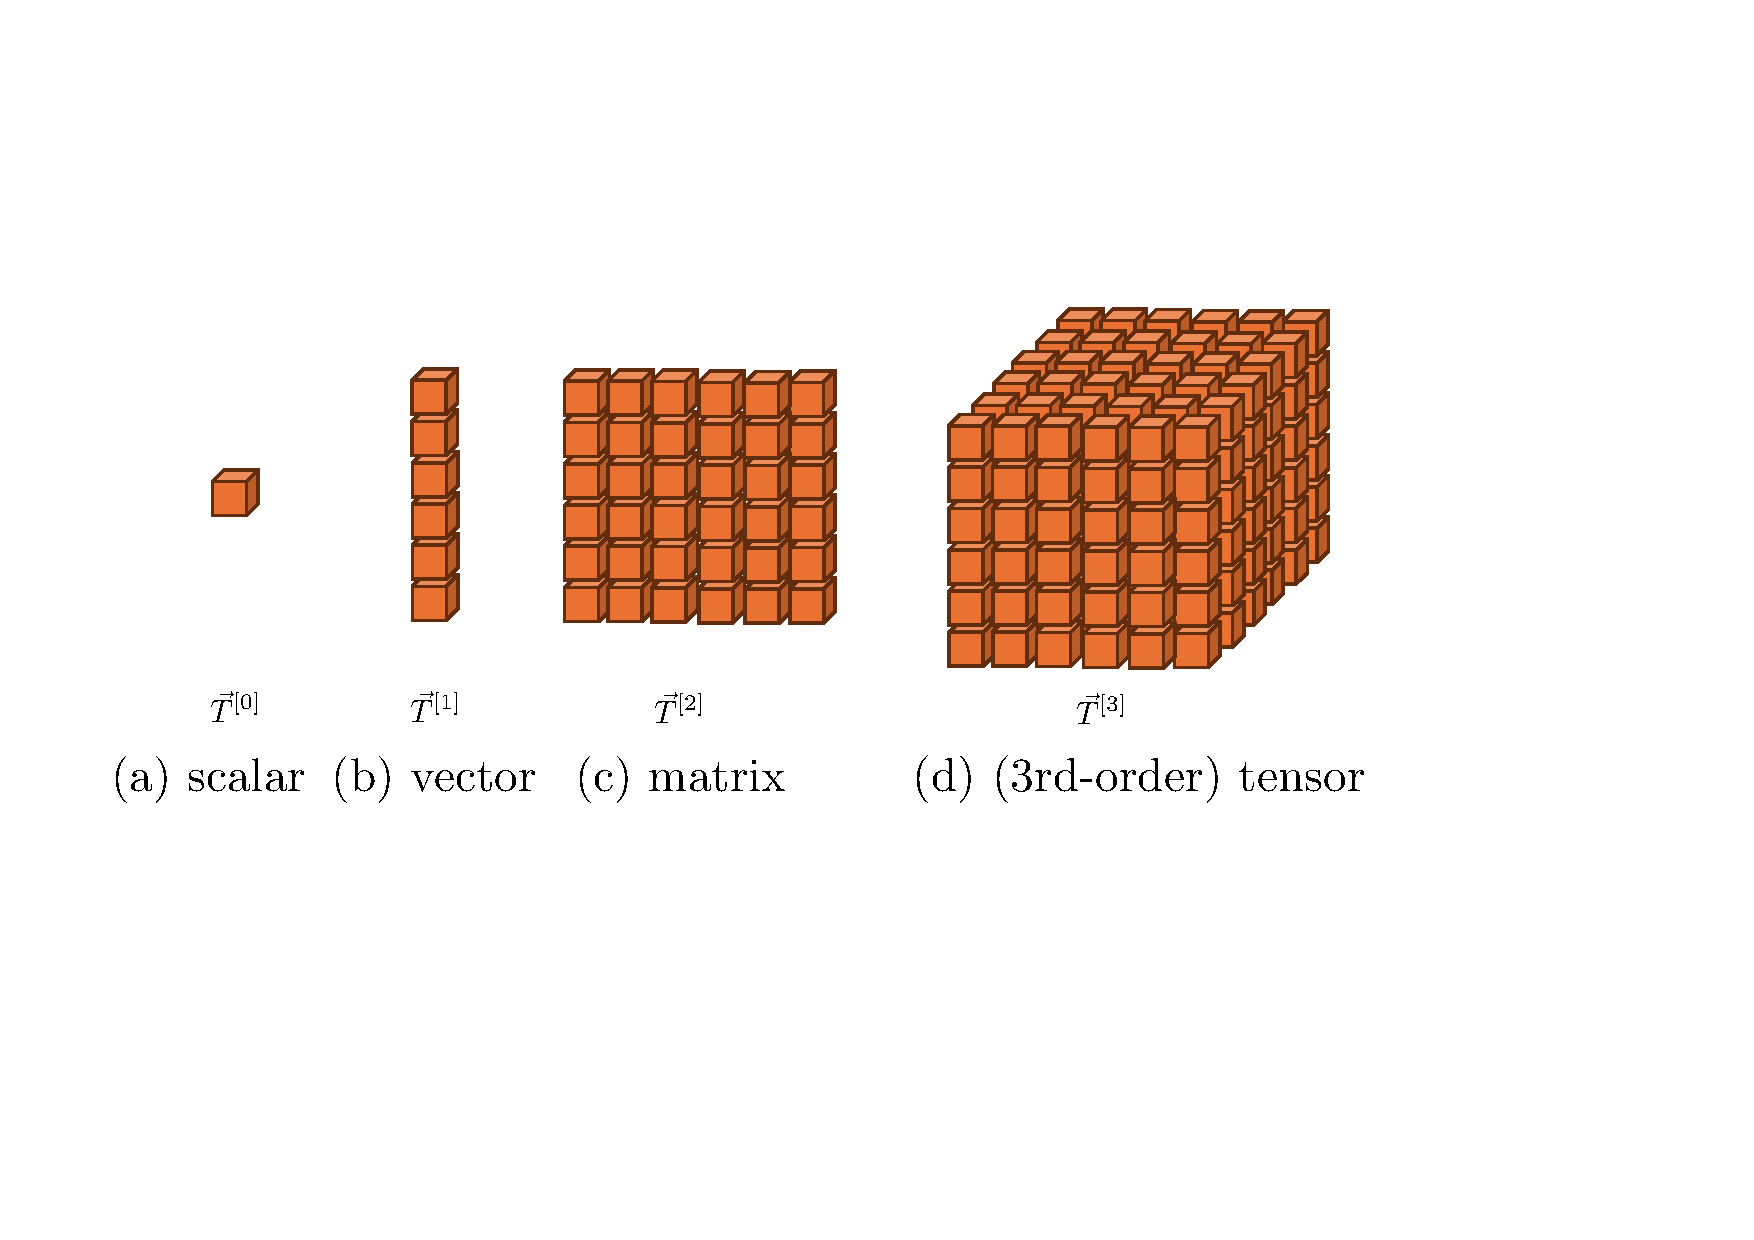
\includegraphics[width=0.6\linewidth]{LA_objects.pdf}

\captionof{figure}{Schematic illustrations of the four key types of \emph{objects} that are of our subject interest, which each one can be considered as a tenor of orders 0 to 3, respectively.}
\label{fig:LA_objects}
\end{minipage}

\hspace{10pt} However, there is no reason why we should stop here, and we can form objects with higher dimensionalities. For example, stacking multiple matrices together we reach a third-order tensor [\cref{fig:LA_objects}] that can be represented by a three-dimensional cube, and we can continue to combine tensor together to form tensors of even higher orders. Following the convention of \citet{duval2023hitchhiker}, we shall denote tensor of order $c$ defined in the Cartesian space as $\vec{T}^{[c]}$,  and it is apparent to see that scalar, vector and matrix are nothing else but tensors of lower ranks of 0, 1 and 2, respectively. 

\hspace{10pt} In physics, the most common ways to express the interactions between two vectors $\bm{v}_1$, $\bm{v}_2\in\mathbb{R}^N$ are achieved by using either the dot product $a=\bm{v}_1\cdot\bm{v}_2$ or the cross product $\bm{b}=\bm{v}_1\times\bm{v}_2$, which returns a scalar $a\in\mathbb{R}$ or a vector $\bm{b}\in\mathbb{R}^{N}$ of the same dimension as the two interacting vectors. However, both these two constructs either preserves the amount of information (as for the cross-product) or significantly loss the information (as for the dot-product) that are encoded in $\bm{v}$, which, however, are often  non-desirable for learning purposes. In the latter case, maximising the information content by encoding more \emph{fine-grained} details on how components in the data interact, thus providing a larger  space to optimise the learning model, is often needed. This can be achieved by using the \textbf{tensor product} to build higher-order tensors from lower ones. For example, consider the tensor product between two three-dimensional vectors $\bm{v}_1=(v_{1x},v_{1y},v_{1z})^\top$ and $\bm{v}_2=(v_{2x},v_{2y},v_{2z})^\top$, the tensor product between them gives back a rank-2 tensor which is a $(3\times3)$ matrix:
\begin{equation}
   \label{eq:tensor_product_two_vector_3D} \bm{v}_1\otimes\bm{v}_2=\left[\begin{array}{ccc}
        v_{1x}v_{2x} & v_{1y}v_{2x} & v_{1z}v_{2x} \\
        v_{1x}v_{2y} & v_{1y}v_{2y} & v_{1z}v_{2y} \\
        v_{1x}v_{2z} & v_{1y}v_{2z} & v_{1z}v_{2z}
    \end{array}\right].
\end{equation}
This shows that the tensor product encodes the mutual interactions between all possible combinations for pairs of elements in $\bm{v}_1$ and $\bm{v}_2$. Generally, (1) the tensor product between two tensors of $c_1$ and $c_2$ gives a higher-order tensor of $c_1+c_2$, (2) one can continues performing tensor products for multiple tensors to encode higher-order information. Following the notation from \citet{willatt2019atom}, the following notation
\begin{equation}
    \label{eq:density_tensor_prod_v}
    \rho^{\otimes \nu} = \underbrace{\rho\otimes\rho\otimes\cdots\otimes\rho}_{\nu}
\end{equation}
shall be used to denote the $v$-th order tensor product of atom-centred density, which we shall provided further example to demonstrate how it encodes $(\nu+1)$-body atom-atom interactions in Box II. 

\hspace{10pt} To provide more physical context, one can refer back to the previous discussions on anharmonic vibrations in solids [\cref{sec:anharmonic_vibs}], the second- ($\boldsymbol{\Phi}_{ij}^{\alpha\beta}$), third-  ($\boldsymbol{\Phi}_{ijk}^{\alpha\beta\gamma}$) and fourth- ($\boldsymbol{\Phi}_{ijkl}^{\alpha\beta\gamma\delta}$) as in \cref{eq:higher_order_vib_Hamiltonian} are all tensors that encodes the information on how pair, triplets and quadruplets of atoms interact when they are independently displaced along a specific Cartesian direction.

\hspace{10pt} Conversely, one can also perform \textbf{tensor contraction} along specific dimension(s) of a higher-order tensor (typically through summations, which can be viewed equivalently as a process of information compression), to generate lower-order tensor. Using again the example given in \cref{eq:higher_order_vib_Hamiltonian}, the operation that involves the fourth-order tensor (which was written in the form of \emph{Einstein summation}), collapse the repeated indices in the tensor product to return a vector as a result:
\begin{equation*}
    \underbrace{\boldsymbol{\Phi}_{ijkl}^{\alpha\beta\gamma\delta}\Delta\bm{R}_l^\delta\Delta \bm{R}_{k}^{\gamma}\Delta\bm{R}_j^{\beta}}_{\mbox{\footnotesize{Einstein summation}}}\equiv\sum_{l\delta}\sum_{k\gamma}\sum_{j\beta}\boldsymbol{\Phi}_{ijkl}^{\alpha\beta\gamma\delta}\Delta\bm{R}_l^\delta\Delta \bm{R}_{k}^{\gamma}\Delta\bm{R}_j^{\beta}=\bm{F}_{i}^{\alpha,(\mathrm{anh},4)},
\end{equation*}
which effectively gives the anharmonic component for the atomic force on atom $i$ along the $\alpha$-direction originated from the fourth order vibration anharmoncity.\cite{yang2021altas}
\end{myquote}


%
% =====================================================
% =====================================================
%

\begin{myquote}
\textbf{Box II: $\rho^{\otimes \nu}$ encodes $(\nu+1)$-body correlations}

\footnotesize

In this box, we shall provide a simplified derivation to showcase, that  applying the tensor products on the atom-centred density fields will enable us to encode the many-body atom-atom correlations in a multiatomic systems, and how this is related to the many body interactions in traditional atom-atom forcefield as discussed in \cref{sect:empirical_forcefield}. 

\hspace{10pt} Starting from the definition of atom-centred density field \cref{eq:atom_env_density_field}, since $\rho_i^{\otimes 1}=\rho_i$, it is apparent that $\rho_i^{\otimes 1}$ encodes two-body information between $i$ and any one of its neighbours $j$. If one integrate out the dependency upon $\bm{r}$
\begin{equation}
    \label{eq:two-body-density-tensor-product-invariant}
    \mathcal{A}(\bm{r}_{ij})=\int\rho(\bm{r}-\bm{r}_{ij})\mathrm{d}\bm{r},
\end{equation}
then we essentially retrieve a quantity that is only dependent on the two-body interactions, resembling the form of the bonding term in atom-atom forcefield.

\hspace{10pt} For the second-order tensor product of $\rho_i$ [\cref{eq:density_tensor_prod_v}], we have
\begin{equation}
    \label{eq:three-body-density-tensor-product}
   \rho_i^{\otimes 2}=\sum_{j \in\mathcal{N}(i)}\sum_{k \in\mathcal{N}(i)}\rho(\bm{r}-\bm{r}_{ij})\rho(\bm{r}-\bm{r}_{ik}),
\end{equation}
which clearly encodes the information amongst a triplet of atoms $(i,j,k)$ in the system. Without going into further mathematical details, we can envisage that such an expression not only contain translational degree of freedom but also an extra one that depends on the relative orientation between the two vectors $\bm{r}_{ij}$ and $\bm{r}_{ik}$, which can be characterised by the bond-angle $\theta_{ijk}=\bm{u}_{ij}\cdot\bm{u}_{ik}/(\Vert \bm{u}_{ij}\Vert\cdot\Vert\bm{u}_{ik}\Vert)$, thus integrating out the translational part in \cref{eq:three-body-density-tensor-product} will lead us to a term $\mathcal{A}(\theta_{ijk})$. One can thus further extend this argument to demonstrate how dihedrals $\varphi_{ijkl}$ may enter in the atom-centred density field representation through $\rho^{\otimes \nu}$ with $\nu=3$, and so on.

%\hspace{10pt} To simplify the mathematical derivations, we shall use the delta function to represent the atom-centred density, such that the density field around a given central atom $i$ can be written as $\rho_i(\bm{R})=\sum_{j\in\mathcal{N}(i)}\delta (\bm{R}-\bm{R}_{j})$. From here, the first-order tensor product of $\rho_i$ [\cref{eq:density_tensor_prod_v}]
%\begin{equation}
%    \label{eq:two-body-density-tensor-product}
%    \rho_i^{\otimes 1}=\sum_{j\in\mathcal{N}(i)}\sum_{k\in\mathcal{N}(i)}\delta (\bm{R}-\bm{R}_j)\delta(\bm{R}-\bm{R}_k),
%\end{equation}
%where in this expression, the centre $i$ is fixed and only the pairs $(j,k)$ can be freely changed to constructed all possible combinations, hence the $\nu=1$ tensor product only encodes 2-body correlations in the system. It can be shown that, if we further takes the averaging over all positions $\bm{R}$  of this tensor product (see Box III), it leads to the following form:
%\begin{equation}
%    \label{eq:two-body-density-tensor-product-invariant}
%    \mathcal{A}(\bm{u})=\int\rho(\bm{R})\rho(\bm{R}+\bm{u}_{jk})d\bm{R},
%\end{equation}
%which depends only upon the interatomic vector $\bm{u}_{jk}$, reflecting the two-body terms in the atom-atom empirical potentials that is usually a function of the bond length.

%\hspace{10pt} Similarly, for the second-order tensor product of $\rho_i$ [\cref{eq:density_tensor_prod_v}]
%\begin{equation}
%    \label{eq:three-body-density-tensor-product}
%    \rho_i^{\otimes 2}=\sum_{j\in\mathcal{N}(i)}\sum_{k\in\mathcal{N}(i)}\sum_{l\in\mathcal{N}(i)}\delta (\bm{R}-\bm{R}_j)\delta(\bm{R}-\bm{R}_k)\delta(\bm{R}-\bm{R}_l).
%\end{equation}
%Following \cref{eq:two-body-density-tensor-product-invariant}, and define $\bm{u}=\bm{R}_j-\bm{R}_k$, $\bm{v}=\bm{R}_l-\bm{R}_k$, with $\theta_{jkl}=\langle\bm{u}\cdot\bm{v}\rangle$ being the angle between $\bm{u}$ and $\bm{v}$, integrating over all vectorial components, we should be able to get
%\begin{equation}
%    \label{eq:three-body-density-tensor-product-invariant}
 %   \mathcal{A}(\theta)=\int %\rho(\bm{R}+\bm{u})\rho(\bm{R})\rho(\bm{R}+\bm{v})\delta(\theta-\theta_{jkl})d\bm{R}d\bm{u}d\bm{v},
%\end{equation}
%which gives a term that only depends on the bond angle amongst a triplet of atoms in the system, and one can simply going further with higher order of $\nu$ to encode the correlations among more combinations of atoms in the system.
\end{myquote}

The next step is to \emph{symmetrise} $\rho^{\otimes \nu}_i$  so it becomes invariant with respect to the rotation of the reference frame, within which the molecular structure is defined. As shown in \textbf{Box III}, for atomistic structures that lives in the space of $\mathbb{R}^3$, the formal way to introduce rotational invariance is by averaging over all copies of $\rho^{\otimes\nu}_i$ that can possibly be generated by operating the rotational operator $\hat{\bm{R}}_{\boldsymbol{\theta}}$ on $\rho^{\otimes\nu}_i$ (for $\nu$ times!), leading to the rotationally averaged atom-centred density field, that is to be denoted with $\overline{\rho^{\otimes \nu}_i}$. Such process of rotational averaging can be achieved through performing the Haar integration on $\rho^{\otimes\nu}_i$.

%
% =====================================================
% =====================================================
%

\begin{myquote}
\textbf{Box III: $\overline{\rho^{\otimes \nu}}$ -- rotational invariance via averaging}

\footnotesize
Physically, the integration procedures as performed in \cref{eq:two-body-density-tensor-product-invariant} is to remove the translational dependent part of the coordinate system in the definitions of the atomic positions, that eventually imposed the important \textbf{translational invariance} in $\mathcal{A}$. Such a procedure is generally referred to as the \emph{\textbf{Haar integration}}, which, in general, for any given quantity $\mathcal{A}$ (in our case, will be a tensorial quantity) where a \textbf{\textit{group action}} $\hat{S}$ upon it will equivariantly transform into a new quantity $\hat{S}\mathcal{A}$, one can obtain a  quantity that is invariant to the transformation of $\hat{S}$ by integrating over all possible $\hat{S}$ acting upon $\mathcal{A}$:
\begin{equation}
    \label{eq:Harr_integration}
    \bar{\mathcal{A}}=\int\hat{S}\mathcal{A}\mathrm{d}\hat{S},
\end{equation}
and a generalisation to the tensor product reads,
\begin{equation}
    \label{eq:Harr_integration_tensor}
    \overline{\mathcal{A}^{\otimes\nu}}=\int\underbrace{\hat{S}\mathcal{A}\otimes \hat{S}\mathcal{A}\cdots\hat{S}\mathcal{A}}_{\nu} \mathrm{d}\hat{S}.
\end{equation}

\hspace{10pt} Returning to the tensor product of the atomic density, and focusing on the term $\rho^{\otimes 1}$, one sees that, after removing the trivial symmetry of translation, the term $\mathcal{A}(\bm{u})$ [\cref{eq:two-body-density-tensor-product-invariant}] is a vector (or rank-1 tensor) property, which is \emph{not} rotationally invariant. In the three-dimensional space, the group that govern the rotation of objects is the \textbf{SO(3) rotation group} [see Box IV], with group action $\hat{\bm{R}}_{\boldsymbol{\theta}}$ that rotates objects in the space (which we shall not worry too much about its concrete form). Based on the about discussion on the Haar integration,  an invariant representation of $\rho^{\otimes 1}$ can thus be constructed as,
\begin{equation}
    \label{eq:two_body_density_rotation_invariance_haar}
    \overline{\rho^{\otimes 1}}=\int_{\mathrm{SO(3)}}\left(\hat{\bm{R}}_{\boldsymbol{\theta}}
    \rho \otimes \hat{\bm{R}}_{\boldsymbol{\theta}}
    \rho\right) \mathrm{d}\hat{\bm{R}}_{\boldsymbol{\theta}},
\end{equation}
which leads to the notation of $\overline{\rho^{\otimes\nu}}$ in the  literatures\cite{willatt2019atom,musil2021physics} that represents the \textbf{symmetrised atom centred density fields}.  As shown in \citet{willatt2019atom}, for a 3D vector, the Haar integration may be evaluated with a suitable parameterisation of the rotation, such as using the Euler angles, and to be computed as
\begin{equation}
    \label{eq:euler_Haar_integration}
    \int_0^{2\pi}\mathrm{d}\alpha\int_0^\pi\sin\beta \mathrm{d}\beta\int_0^{2\pi}\mathrm{d}\gamma \bm{u}(\alpha,\beta,\gamma),
\end{equation}
which one can anticipate that the end result is only dependent on the modulus of $\bm{u}$, \emph{i.e.} $\Vert\bm{u}\Vert_2$.
\end{myquote}

%
% =====================================================
% =====================================================
%

Nevertheless, explicitly performing the Haar integration to obtain $\overline{\rho^{\otimes \nu}_i}$ for every atomistic structure to be investigated will not be numerically efficient.  The mathematical trick that can be used to simplify problem is via the use of group theory (which are further explained in \textbf{Box IV}), particularly, the rotational group in three dimensions, or SO(3), and it further brings the bra-component for constructing atom-centred density field representation into the equation. Practically, this is typically achieved via three steps. Firstly, one projects $\rho_{i}(r)$ on a set of radial $\{R_n(r)\}$ and angular $\{Y_{\ell}^{m}(\hat{\bm{r}})\}$ (where $\hat{\bm{r}}$ denotes a projection of $\bm{r}$ onto a unit sphere) to obtain a set of expansion coefficients $\{c_{n\ell m}\}$ (for $n=1,2,\ldots,m_{\max}$, $\ell=0,1,2,\ldots,\ell_{\max}$ and $m=-\ell,-\ell+1,\ldots,\ell-1,\ell$) in which,
\begin{equation}
    \label{eq:soap_expansion_coeff}
    c_{n\ell m}:=\langle n\ell m|\rho_i(\bm{r})\rangle=\int R_{n}(r)Y_{\ell}^{m}(\hat{\bm{r}})\rho(\bm{r})\mathrm{d}\bm{r}.
\end{equation}
Collecting $\{c_{n\ell m}\}$ leads to a vector of expansion coefficients $\bm{c}$. The radial basis functions are typically chosen as $n$ Gaussian functions with equi-distant centres positioned in the interval $[0,r_c]$. The radial components are generally invariant and hence one only needs to focus on symmetrising the angular part in the second step.
Using the SOAP descriptor as example, $\rho^{\otimes2}_i$ can be directly obtained by performing the tensor product of $\bm{c}\otimes\bm{c}$, which gives a combination of rank-2 tensors with dimensions from $(0\times0)$ up to $(\ell_{\max}\times\ell_{\max})$ where the tensor elements can be written as $c_{n_1\ell_1 m_1,n_2\ell_2 m_2}:=\langle n_1\ell_1 m_1,n_2\ell_2 m_2 |\rho^{\otimes 2}_i\rangle=c_{n_1\ell_1 m_1}c^{*}_{n_2\ell_2 m_2}$ [\cref{eq:tensor_prod_decomp_general}]. For the na\"{i}ve SOAP descriptor,\cite{bartok2013representing} in which we are  interested in the rotationally invariant part of the tensor product, only the entries with $\ell_1=\ell_2$ are relevant, and invariance can be further imposed by summing over the magnetic quantum numbers for a given $\ell$, leading to the so-called SOAP spectrum representation:
\begin{equation}
\label{eq:SOAP_spectrum}
\chi_{n_1n_2\ell}=\sum_{m=-\ell}^{\ell}c_{n_1\ell m}c^{*}_{n_2\ell m},
\end{equation}
(or equivalently as $\langle n_1n_2\ell|\overline{\rho^{\otimes 2}_i}\rangle$),
whereby the final SOAP structural descriptor for a given centre $i$ (or $\boldsymbol{\chi}_i$) is constructed by concatenating  $\chi_{n_1n_2\ell}$ for this centre with all combinations of $(n_1,n_2,\ell)$. The global descriptor for a structure containing $N$ atoms can thus be constructed by further concatenating $\boldsymbol{\chi}_i$ as $[\boldsymbol{\chi}_1,\boldsymbol{\chi}_2,\ldots,\boldsymbol{\chi}_N]^\top$. This thus concludes our short discussions on the philosophy behind the designs of invariant SOAP structural descriptors. 
 
\begin{myquote}
    \textbf{Box IV: simplifying the computation of density-based representation with group theory}

\footnotesize
\hspace{10pt} One can envisage that, explicitly computing the integral such as \cref{eq:two_body_density_rotation_invariance_haar} to achieve rotational invariance will be numerically expensive, and applying the knowledge of group theory, in this case, the SO(3) rotational group in $\mathbb{R}^3$, will allow us to break down the rotation into its elementary building blocks, which are called the \emph{irreducible representations (irreps)}, that can be more easily manipulated independently. 

\hspace{10pt} Rather than treating the abstract object of atom-centred density $\rho$, we shall focus our discussion using more concrete examples of tensors (which will also become relevant to the subsequent discussions on equivariant NNs). For this, we start from a rank-1 tensor $\hat{T}^{[1]}\in\mathbb{R}^{3}$ defined in the Cartesian space, and tensors of higher ranks $\hat{T}^{[\nu]}$ can be constructed using tensor products as outlined in Box I. In this case, rotation of tensors of different ranks can be achieved by repeatedly applying the rotational operators, for examples:
\begin{align*}
    \rho^{\otimes 1}\sim\hat{T}^{\prime [1]}&\leftarrow \hat{\bm{R}}_{\boldsymbol{\theta}}\hat{T}^{[1]},\\
    \rho^{\otimes 2}\sim\hat{T}^{\prime [2]}&\leftarrow 
    \hat{\bm{R}}_{\boldsymbol{\theta}}\hat{\bm{R}}_{\boldsymbol{\theta}}\hat{T}^{[2]}, \\
    \rho^{\otimes 3}\sim\hat{T}^{\prime [\nu]}&\leftarrow \underbrace{\hat{\bm{R}}_{\boldsymbol{\theta}}\hat{\bm{R}}_{\boldsymbol{\theta}}\cdots\hat{\bm{R}}_{\boldsymbol{\theta}}}_{\nu}\hat{T}^{[\nu]}.
\end{align*}
Several key observations should be noted here: (1) Tensors of different types (indicated by their order $\nu$) transform differently, as characterised by the number of times that the operator $\hat{\bm{R}}_{\boldsymbol{\theta}}$ is applied. (2) Repeatedly performing the product operations to rotate higher-order tensors will not be computationally efficient. Following the pedagogical introductions in \citet{duval2023hitchhiker}, group theory gives us a mathematical tool to \emph{decompose} a higher-order tensor $\hat{T}^{[\nu]}$ into the linear combination of \emph{irreps} (thus only summation operations are required), which are the \emph{orthogonal basis} for the SO(3) rotational group. These basis are of the form of tensors themselves, which also follow their own transformation rules that depend on their ranks (dubbed as $\ell$, which is the \textit{angular momentum quantum number} in quantum mechanics), but in this case, can be achieved with a single (basis specific) Wigner D matrix, denoted as $\mathbf{D}^{\ell}(\hat{\bm{R}}_{\boldsymbol{\theta}})$).

\hspace{10pt} As a concrete example (see more detailed derivation in \citet{duval2023hitchhiker}), the decomposition of $\hat{T}^{[2]}$ (that is a tensor product between two vectors in $\mathbb{R}^3$) can be written as:
\begin{equation}
    \label{eq:rank_2_tensor_decomp}
    \vec{T}_1^{[1]}\times\vec{T}_2^{[1]}\to\vec{T}^{[2]} = \lambda_1\cdot \underbrace{\hat{T}_1^{[2]}}_{\ell=0}+\left[ \begin{array}{c}
         \lambda_2  \\
         \lambda_3 \\
         \lambda_4
    \end{array} \right] \cdot \underbrace{\left[ \begin{array}{c}
         \hat{T}_2^{[2]} \\
         \hat{T}_3^{[2]}  \\
         \hat{T}_4^{[2]} 
    \end{array} \right]}_{\ell=1} + \left[
    \begin{array}{c}
         \lambda_5  \\
         \lambda_6 \\
         \lambda_7 \\
         \lambda_8 \\
         \lambda_9
    \end{array} \right] \cdot \underbrace{\left[ \begin{array}{c}
         \hat{T}_5^{[2]} \\
         \hat{T}_6^{[2]}  \\
         \hat{T}_7^{[2]} \\
         \hat{T}_8^{[2]} \\
         \hat{T}_9^{[2]}
    \end{array} \right]}_{\ell=2}
\end{equation}
in which we use the symbol $\hat{T}^{[2]}_i$ to specify the $i$-th basis that is a rank-2 tensor. This shows that $\vec{T}^{[2]}$ can be decomposed into 9 basis of $\hat{T}^{[2]}_i$ [which is consistent with the number of elements in the matrix form of $\vec{T}^{[2]}$, see \cref{eq:tensor_product_two_vector_3D}]. These basis  can be further grouped depending on $\ell$, which leads to the sum as expansions in the 1, 3, and 5 dimensional spaces, expressed as tensor basis of ranks 0, 1 and 2, respectively, or more compactly as $1\otimes1=0\oplus1\oplus2$. In general, for the tensor products between two tensors of rank $\ell_1$ and $\ell_2$, we have:
\begin{equation}
    \label{eq:tensor_prod_decomp_general}
    \ell_1\otimes\ell_2=\bigoplus_{|\ell_1-\ell_2|}^{\ell_1+\ell_2}\hat{T}^{[\ell]}.
\end{equation}
Finally, collecting the expansion coefficients $\lambda$'s according to $\ell$ into a vector, and following the conventional notation of magnetic quantum numbers $m_\ell\in\{-\ell,-\ell+1,\cdots,\ell-1,\ell\}$, that gives $\vec{\lambda}^{(\ell)}=\left[\lambda^{(\ell)}_{-\ell},\lambda^{(\ell)}_{-\ell+1},\ldots,\lambda^{(\ell)}_{\ell-1},\lambda^{(\ell)}_{\ell}\right]^\top$, then the rotation of the rank-2 tensor product can be achieved in the following additive form, which is the result if we work with \textbf{\textit{finite dimensional representation theory}}:
\begin{equation}
    \label{eq:Wigner_D_matrix_rotate_rank_2_tensor}
    \hat{\bm{R}}_{\boldsymbol{\theta}}\hat{\bm{R}}_{\boldsymbol{\theta}}\vec{T}^{[2]} = \bm{D}^{(0)}(\hat{\bm{R}}_{\boldsymbol{\theta}})\vec{\lambda}^{(0)}\oplus \bm{D}^{(1)}(\hat{\bm{R}}_{\boldsymbol{\theta}})\vec{\lambda}^{(1)}\oplus \bm{D}^{(2)}(\hat{\bm{R}}_{\boldsymbol{\theta}})\vec{\lambda}^{(2)}.
\end{equation}

\hspace{10pt} Is this the best solution? Not necessarily! Firstly, one is yet to perform rotational average over the Wigner D-matrices to achieve rotationally invariance. Secondly, particularly for encoding interactions in NNs through tensor products, it does not seems efficient to perform tensor decomposition after every tensor product operations, as the possible number of tensor products to handle can be extremely large. Finally, one may also question whether the use of a finite basis to decompose rotation can sufficiently encode finite orientational details in molecular modelling (\emph{e.g.} in the case of continuous geometric change during MD simulations). The alternative approach, as more widely adopted in both descriptor-based ML\cite{bartok2013representing,drautz2019atomic} and equivariant neural networks\cite{duval2023hitchhiker} is to harness the \textbf{spherical harmonics} $\{Y_{\ell}^{m}\}$ as the \emph{\textbf{infinite dimensional basis set}}, to first expand the angular part of the (uncorrelated) atom-centred density $\rho(\bm{r})$ and then construct higher-order invariant and/or equivariant features from it. 

\hspace{10pt} In the subsequent discussions, we focus on the angular part of the density field $\rho(\bm{r})$, assuming it has been projected on to the surface of the unit sphere in $\mathbb{R}^3$, thus the radial part can be temporarily discarded. In this case,   $\rho(\bm{r})$ (a rank-1 vector) can be expanded in the basis of spherical harmonics as 
\begin{equation}
    \label{eq:sph_expand_density}
    \rho_i(\bm{r})=\sum_{\ell m}c_{\ell m}Y_\ell^m (\bm{r}),
\end{equation}
up to a predefined hyperparameter of $\ell_{\max}$. Similar to $\vec{\lambda}^{(\ell)}$, the expansion coefficients $c_{\ell m}$ can be grouped into tensors of different orders of $\ell$, which may be denoted as $\vec{c}^{(\ell)}$. Using the bra-ket notation from Dirac's formulations of quantum mechanics, that is also adopted in the literatures of density-based structural representations,\cite{willatt2019atom} we can compute $c_{\ell m}=\langle\ell m|\rho_i\rangle$, which projects an abstract density onto a concrete representation as denoted by the state of $|\ell m\rangle$. At the limit of the $\delta$-function-like density field, $c_{\ell m}\leftarrow \sum_j Y_{\ell m}(\bm{r}_{ij})$ (\emph{c.f.} Steinhardt order parameters\cite{steinhardt1983bond}), thus can be easily computed from the interatomic vector. In this case, collecting the expansion coefficients 
\begin{equation}
    \label{eq:expansion_coeff_vector_sph}
    \vec{\bm{c}}=\left[\vec{c}^{(0)},\vec{c}^{(1)},\ldots,\vec{c}^{(\ell_{\max})}\right]
\end{equation}
leads to a \emph{representation} that encodes the angular information of the density field, which is yet to be symmetrised. 

\begin{minipage}[t]{\linewidth}

\centering
\includegraphics[width=0.75\linewidth]{soap_invariant_tensor_prod.pdf}

\captionof{figure}{Illustration of the construction for the (only the angular part) of the SOAP descriptor, starting from tensor product of two list of tensors consisting the expansion coefficients (left). The tensor product leads to a range of multiple tensors, which we arrange into a two-dimensional matrix form (middle), where the final SOAP descriptor comes from extracting only the diagonal part ($\ell_1=\ell_2$) followed by summing over the magnetic quantum number $m$ for a given $\ell$ to retain invariance. }
\label{fig:soap_invariant_tensor_prod}
\end{minipage}

\vspace{10pt}

\hspace{10pt} To proceed, the second-order tensor product between atom-centred density fields can now be computed through the tensor product $\rho^{\otimes 2}\sim\vec{\bm{c}}\otimes\vec{\bm{c}}$, which in terms we need to form tensor products between all possible pairs of tensors $\vec{c}^{(\ell_1)}\otimes\vec{c}^{(\ell_2)}$ in $\vec{\bm{c}}$ with $\ell_1,\ell_2\in[0,\ell_{\max}]$, leading to a set of multiple tensors (each of the rank $\ell_1+\ell_2$), as shown in the middle section of \cref{fig:soap_invariant_tensor_prod}. As indicated in \cref{eq:tensor_prod_decomp_general}, each one of these tensors can be further decomposed into a sum of tensors with ranks from $|\ell_1-\ell_2|$ to $(\ell_1+\ell_2)$, which is usually expressed as $\ell_1\otimes\ell_2=|\ell_1-\ell_2|\oplus|\ell_1-\ell_2|+1\oplus\cdots\oplus \ell_1+\ell_2$.  Another important point, which will becomes useful later, is that each decomposed tensor do not contribute to the sum equally, but is weighted by some coefficients, known as the \textbf{\textit{Clebsh-Gordan (CG) coefficients}}. In the case of $\rho^{\otimes 2}$, we have
\begin{equation}
    \label{eq:CG_decomposition}
    \rho^{\otimes 2}_i\sim\sum_{LM}\sum_{\substack{\ell_1 m_1\\ \ell_2 m_2}}C^{LM}_{\ell_1 m_1\ell_2 m_2}c_{\ell_1 m_1}c_{\ell_2 m_2},
\end{equation}
in which the CG coefficient $C^{LM}_{\ell_1 m_1\ell_2 m_2}$ is defined based on the combinations of $(\ell_1,\ell_2)$ and $(m_1,m_2)$ that can lead to the decomposed tensor element with $L\in[|\ell_1-\ell_2|,\ldots,\ell_1+\ell_2]$ and $M\in[-L,\ldots,L]$.

\hspace{10pt} At this moment, we are only interested in retrieving the invariant components $L=0$ to construct the final SOAP descriptor,\cite{bartok2013representing} so we will only be interested in the tensor products $\vec{c}^{(\ell_1)}\otimes\vec{c}^{(\ell_2)}$ with $\ell_1=\ell_2=\ell$ and extract only the decomposed component with $L=0$. (In the SO(3) group theory language, we say there exists only one \emph{pathway} to combine $\ell$'s that gives $L$, in this case, the only relevant CG coefficient in \cref{eq:CG_decomposition} is left with $C^{0M}_{\ell m_1\ell m_2}$.) From here, it is obvious that $\vec{c}^{(\ell)}\otimes\vec{c}^{(\ell)}$ is a rank-2 tensor with the dimension of $((2\ell+1)\times(2\ell+1))$, and matrix element $c_{\ell m_1}c_{\ell m_2}$. Without going into further mathematical details, we can intuitively understand that, a practical way to extract a scalar (thus invariant) component of the tensor can be achieved by taking the trace of this rank-2 tensor, leading to the final construct of the SOAP descriptor (angular part only, rightmost of \cref{fig:soap_invariant_tensor_prod}):
\begin{equation*}
\chi_{\ell}=\sum_{m}c_{\ell m}c^{*}_{\ell m},
\end{equation*}
which here we put the complex conjugate back, as in the original formulation\cite{bartok2010gaussian} to signify that the spherical harmonic basis are complex numbers.

%\hspace{10pt} Now, going on to the next step, for a given coefficient $c_{\ell m}\in\{c_{\ell m}\}_{m=-\ell}^\ell$,  \cref{eq:Wigner_D_matrix_rotate_rank_2_tensor} tell us, under rotation, it transform as $c_{\ell m}^\prime\leftarrow \sum_{m^\prime} D_{mm^\prime}^{(\ell)}(R)c_{\ell m^\prime}$, which will mix different $m$ together for a given $\ell$. 

\end{myquote}

At this point, it is natural to think about following the above recipe to construct many-body correlations $\rho^{\otimes \nu}_i$ ($\nu>2$) that accounts for more complex multiatomic interactions that may contribute to the total energy of the system, that is in line with the expansion scheme introduced in \cref{eq:total_energy_atom_pos_expand}. A particular example is for the modelling of solid-state materials within the conceptual framework of the embedded atom scheme [as introduced in \cref{sect:empirical_forcefield}] where all the surrounding atoms around the central atom can mutually interact with each other. However, the na\"{i}ve way of the computing the tensor product and extracting the invariant components, as explained in \textbf{Box IV} become practically intractable for higher-order terms. Considering, for example $\rho^{\otimes 3}_i$, which, following \cref{eq:CG_decomposition}, we should have (following the ACE notation where $A_{n\ell m}=\langle n\ell m|\rho_{i}\rangle$):
\begin{equation}
    \label{eq:CG_decomposition_3rd_order}
    \rho^{\otimes 3}_i\sim\sum_{\substack{\ell_1 m_1\\ \ell_2 m_2\\ \ell_3 m_3}}C^{00}_{\ell_1 m_1\ell_2 m_2 \ell_3 m_3}A_{\ell_1 m_1}A_{\ell_2 m_2}A_{\ell_3 m_3}.
\end{equation}
Focusing only on the invariant part thus enforcing $\ell_1\otimes\ell_2\otimes\ell_3\to0$, one can see there are multiple pathway to select the combinations of $\ell_i$ and $m_i$ (i=1,2,3) to achieve this outcome. For example, considering the case with $\ell_1=\ell_2=\ell_3=2$, we may first combine $\ell_1\otimes\ell_2=0\otimes1\otimes2\otimes3\otimes4$, in which only $\ell_3=2$ can be combined with the $\ell_1\otimes\ell_2=2$ (which will be denoted as $L_{12}$ and correspondingly $M_{12}$) component to obtain $L=0$. However, now with $M_{12}\in[-2,2]$ and $m_3\in[-2,2]$, we have five combinations of $(M_{12},m_3)$ that can lead to the final outcomes of $M=0$, which are $(-2,2)$, $(-1,1)$, $(0,0)$, $(1,-1)$ and $(2,-2)$. One can easily envisage that this can soon become a book-keeping exercise that, the above approach, that aim to surrogate higher-order body correlations based on the uncoupled basis of $\{A\}$, is prone for errors for large $\nu$. The ACE framework, as formulated by \citet{drautz2019atomic}, is to first replace the uncoupled basis $\{A\}$ with a coupled basis $\{B^{(\nu)}\}$ that is formed by first summing over all combination of indices that fulfil the condition of $\sum_{i=1}^{\nu}m_{i}=0$, for example, in the cases of $\rho^{\otimes \nu}$ with $\nu=0,1,2$, it leads to 
\begin{subequations}
\label{eq:ACE_basis}
\begin{align}
    B_{in}^{(1)}&=A_{in00},\label{eq:ACE_1_basis}\\
    B_{in_1 n_2\ell}^{(2)} &=\sum_{m=-\ell}^{\ell}(-1)^m A_{in_1\ell m}A_{in_2\ell -m},\label{eq:ACE_2_basis}\\
    B_{\substack{in_1 n_2 n_3\\ \ell_1 \ell_2 \ell_3}}^{(3)} &= \sum_{m_1=-\ell_1}^{\ell_1}\sum_{m_2=-\ell_2}^{\ell_2}\sum_{m_3=-\ell_3}^{\ell_3}\left(\begin{array}{ccc}
        \ell_1 & \ell_2 & \ell_3\\
         m_1 & m_2 & m_3
    \end{array}\right)A_{in_1\ell_1 m_1}A_{in_2\ell_2 m_2}A_{in_3\ell_3 m_3}, \label{eq:ACE_3_basis}
\end{align}
\end{subequations}
in which the coefficients in \cref{eq:ACE_3_basis} are given in the Wigner $3j$ symbol. With this construct, the part of the total system energy in \cref{eq:total_energy_atom_pos_expand} that is contributed from the $i$-th central atom interacting with its surrounding environment (\emph{i.e.} the cluster $\boldsymbol{\sigma}$ around $i$), can be expressed in the $B$-basis without invoking the tensor product among $B$'s:
\begin{equation}
    \label{eq:ACE_atom_energy_expansion}
    E_i(\boldsymbol{\sigma})=\sum_{n}c_n^{(1)}B_{in}^{(1)}+\sum_{n_1n_2\ell}^{\prime}c_{n_1 n_2\ell}^{(2)}B_{in_1 n_2\ell}^{(2)}
    +\sum_{\substack{n_1 n_2 n_3\\ \ell_1 \ell_2 \ell_3}}^{\prime}c_{\substack{n_1 n_2 n_3\\ \ell_1 \ell_2 \ell_3}}^{(3)}B_{\substack{in_1 n_2 n_3\\ \ell_1 \ell_2 \ell_3}}^{(3)}+\cdots,
\end{equation}
where $c^{(\nu)}$ are no longer fixed expansion coefficients but learnable coefficients for fitting the ML interatomic potentials. With such a construction, it can be shown that the complexity of computing the $(\nu+1)$-body correlation features can be significantly reduced from that of $\mathcal{O}((2\ell+1)^\nu)$ for na\"{i}ve SOAP to that of $\mathcal{O}(\nu(2\ell+1)^2)$ for ACE with a given $\ell$. 



\begin{figure}[htb]
    \centering
    \includegraphics[width=\linewidth]{binding_curve_soap_longrange.png}
    \caption{Median-error binding curves for molecular dimers across six different classes of intermolecular interactions. (black lines) Quantum-mechanical calculations. (green lines) Predictions with the SOAP descriptor constructed based on the $\left\vert \overline{\rho_i\otimes\rho_i}\right\rangle$ model. (blue lines) Predictions based on a $\left\vert \overline{\rho_i\otimes V_i}\right\rangle$ models that takes into account for the long-ranged interactions [adopted from \citet{grisafi2021multi}].}
    \label{fig:binding_curve_soap_longrange}
\end{figure}

\textbf{\emph{Interpretability of descriptor-based ML models}} Before we conclude this part that has discussed the physics-inspired constructions of the atom density field representations for atomistic structures for ML, we would like to briefly account on how the descriptor-based ML  generally lead to better model interpretability. At the very first place, as shown in \cref{appendix:supervised_ML} and \ref{appendix:unsupervised_ML}, the underlying ML models are usually quite simple in terms of the mathematical operations that are to be performed on the input data in order to reach the target output are generally very simple, mostly linear operations. The possible existence of the complex nonlinearity is handled by the constructions of the similar kernel matrix (or equivalently, in the context of atom density field representations, the structural descriptors). As mentioned above, such a principled model design is already based on a strong physical prior on our fundamental understandings on the structural-property relationships for materials, in which similar materials should adopt similar properties. 

On the other hand, such design also implies that, the predictive accuracy of supervised ML model or the insightfulness of the unsupervised ML model, will be predominantly determined by the quality of the descriptors that are hand-crafted based on the specific domain knowledge that underpins the specific problems to be solved at hand. As seen above, such knowledge entails the structural, physical and/or physical properties of the datasets, that may additionally include the incorporations of constraints, such as symmetries in the case of structural descriptors, to enable efficient learnings. This is critical when it comes to asking the question on which set of factors contributes strongly to specific properties for the materials, or conversely, what features might be lacking that are critically needed for improving the predictive accuracy of the model. For example, as shown in \cref{fig:binding_curve_soap_longrange} when it comes to the long-ranged noncovalent interactions between molecular fragments,\cite{grisafi2021multi} simply using the density field $\overline{\rho_i^{\otimes 2}}$ that is constructed from the neighbouring atoms identified based on a pre-defined cut-off radius $r_c$ leads to early plateauing thus no able to surrogate the full quantum-mechanical binding curve for the molecular dimers. This naturally leads to one proposal (of, possibly many others) to improve the SOAP model by augmenting $\rho_i$ with a Coulomb-type long-range potential:
\begin{equation*}
    |\rho\otimes V\rangle\sim\int \mathrm{d}\bm{x}^\prime \frac{|\rho\rangle}{|\bm{x}-\bm{x}^\prime|},
\end{equation*}
with which one is able to arrive at the ML predicted binding curves that closely follows that of the quantum-mechanical ones. Model development efforts as such can draw parallel comparison to those earlier endeavours on the development of polarisable forcefields [\cref{sect:polarisable_FF}] that both aim to capture how long-range electrostatic interactions and chemical environments interdepend on each other.

It is therefore clear, that, the descriptor-based ML represents a paradigm in which the designs and optimisations of the materials representations are, in principle, separated from the optimisations of the actual learning algorithm, which is distinctively different from the deep learning approaches to be discussed in the next section. This means that the descriptors are fixed prior to, and not further optimised, during the model learning process, which may otherwise leads to a new set of features in the model's latent space that are significantly different from the initial input, highlighting other sets of features of the training data that may not be immediately apparent on what these features really are. In this case, the use of hand-crafted descriptors becomes particularly helpful when it comes to enhancing the model's interpretability, especially many hyperparameters that control the computations of the descriptors bear strong physical meaning, such as the cut-off radius ($r_c$, controlling how far apart a central atom can see its neighbours) and the many-body order ($\nu$, controlling the maximal number of interacting neighbouring atoms), in the construction of the SOAP-type structural descriptors.
